\chapter{Deliverable}
\label{chap:deliverable}
This section presents the solution, the testing and evaluation processes conducted to validate the KU-Eater system and measure its usability from actual users' perspectives.

\section{Software Solution}
\label{section:software-solution}
The software is hosted in the GitHub platform within organization the same name as our project.\footnote{\url{https://github.com/KU-Eater}}
The project consists of four different components:
\begin{itemize}[leftmargin=40pt]
    \item \textbf{Protocol} is a gRPC protocol definition repository, where we can share data schema and use gRPC to auto generate stubs when working between all services.
    \item \textbf{Agent} is a recommendation generator and embedder running our model. It uses Sentence Transformers and gRPC protocol to communicate with the backend.
    \item \textbf{Backend} is a backstage of our project. It contains a Rust-based server that boasts in speed. The server also communicates using gRPC and gRPC-Web.
    \item \textbf{Frontend} is the canvas of our project. It is built on React Native and Typescript.
\end{itemize}

The screenshots of KU Eater is found at \ref{appendix:B}.

\section{Test Report}
\label{section:test-report}
The process consists of two main parts:

\subsection{Manual Testing}
\label{subsection:manual-test}
Manual testing was carried out based on the user stories defined in the project backlog. Each test case was designed to verify a core feature of the system such as login, viewing menus, saving favorites, and submitting reviews. The test cases include the test name, test steps, expected results, and actual outcomes (Pass/Fail). In this report, 5–6 key test cases will be presented, while the complete test case table is provided via the footnote\footnote{\url{https://docs.google.com/spreadsheets/d/1h3U8jayLPo5yrrw5xFO60UDDK73uBKbyfsefvP32nKk/}}

\begin{figure}[h!]
    \centering
    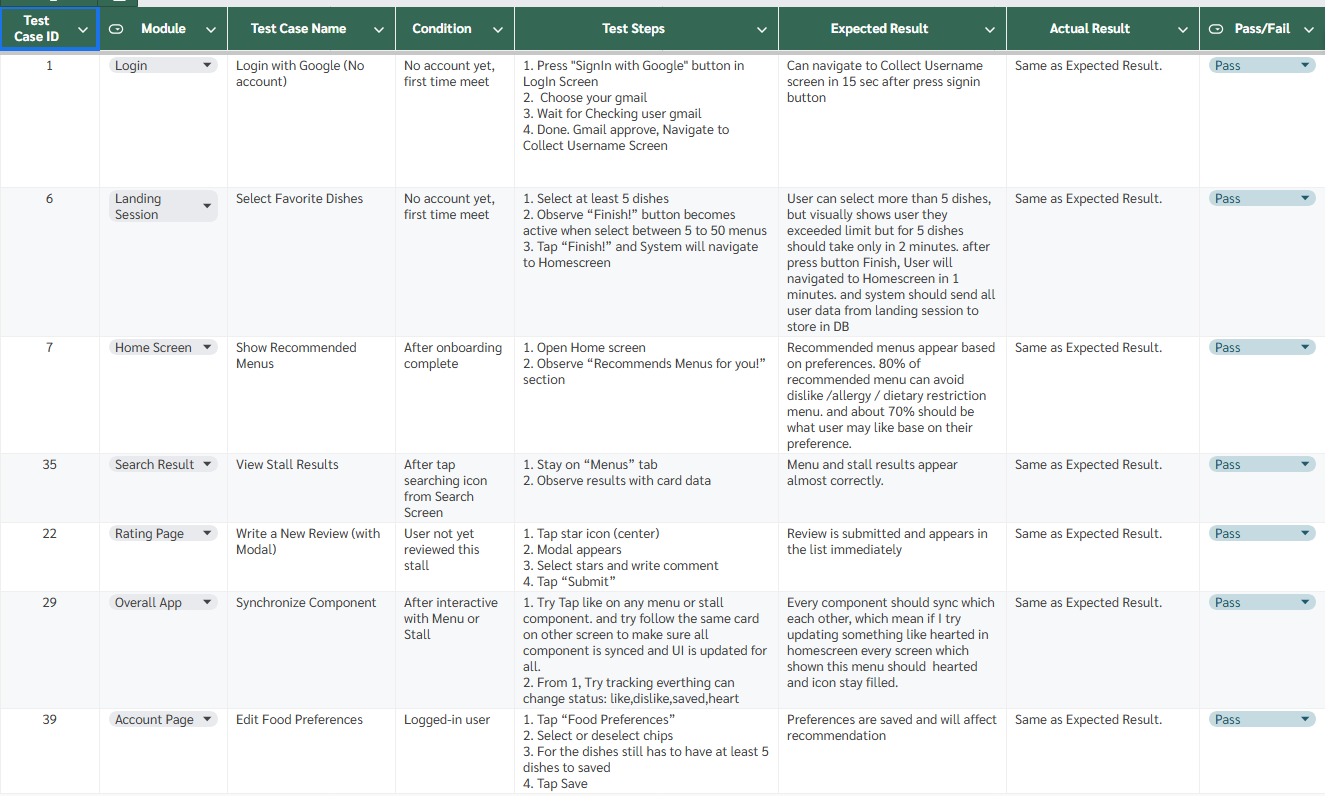
\includegraphics[width=\textwidth,height=0.5\textheight,keepaspectratio]{kueater/manual-testing.png}
    \caption{Table of Manual Testing}
    \label{fig:manual-testing}
\end{figure}

\subsection{User Evaluation Questionnaire}
\label{subsection:questionnaire}
In addition to technical testing, a user evaluation questionnaire was conducted to measure user satisfaction and perceived usability before and after using the system. The full questionnaire consists of 21 questions, but around 10 relevant questions are selected to be summarized in this chapter. The results are presented in graphical format for ease of analysis and interpretation.

To evaluate the effectiveness of KU-Eater and its impact on the user experience, a questionnaire was created and distributed using Google Forms. The primary objective of this evaluation is to assess how well the system improves the food selection experience in Kasetsart University cafeterias. The form comprised 21 questions, categorized into five key areas aligned with the system's core features and intended outcomes:

\begin{itemize}[leftmargin=80pt]
    \item Before vs After usage comparison
    \item Search functionality
    \item Recommendation system
    \item Review and rating feature
    \item Overall user satisfaction and suggestions
\end{itemize}

\subsection{Evaluation Results}
\label{subsection:evaluation-results}

\textbf{Recommendation Accuracy}

Participants were asked to rate the accuracy of KU-Eater's recommended menus and stalls. Approximately 78\% of respondents found the
recommendations to be either “quite accurate” or “very accurate,” while only 7\% rated 
them as “not very accurate.” Notably, no participants selected “not accurate at all.”

These results in \ref{fig:recommendation-accuracy} suggest that the system's recommendation engine is generally perceived as reliable and relevant to users' personal preferences.

\textbf{Ease of Finding Menus}

To assess the impact of the search feature, users were asked to rate how easy it was to find desired menus before and after using KU-Eater.
The average ease score increased significantly, from 23\% before using the app to 73\% afterward.
Additionally, 78\% of users reported that the app made it easier to find menus, while 21\% experienced no noticeable difference.

These findings in \ref{fig:ease-of-finding} indicate that the search feature provides tangible benefits in reducing the effort needed to locate specific dishes or stalls.

\textbf{Review and Rating Feature}

When asked whether food reviews within the application influenced their decisions, 79\% of users agreed that the reviews were impactful while 
42.86\% selected “very influential” and 35.71\% chose “quite influential.” Importantly, none of the participants rated the reviews as unhelpful. 

However, when asked about their own likelihood of writing reviews, only 43\% indicated that they were
likely or very likely to contribute. This discrepancy highlights a common behavioral gap: while users benefit from others' reviews,
they are less inclined to write their own.

These insights (\ref{fig:influenced-by-review}, \ref{fig:likelihood-to-write}) suggests that the review feature
could be improved by making the review process easier or more engaging to encourage user participation.

\textbf{Most Liked Features}

Users were asked to select which features of KU-Eater they liked the most. The top three features were the recommendation system
(78.57\%), the easy-to-use interface (71.43\%), and the search functionality (64.29\%). Other well-received features
included the review system, saved lists, and customizable preferences.
These results from \ref{fig:most-liked-features} demonstrates that users value a balance between intelligent recommendations, simplicity in design, and tools that allow personalization and feedback.

\textbf{Decision-Making Speed}

Users were also asked whether KU-Eater affected the time it took them to decide what to eat. Over 71\% of participants stated that
their decision-making speed improved, with 43\% reporting a slightly faster experience and 29\% stating
it was much faster. The remaining 29\% observed no change, and no participants reported that the app made the
process slower. This (\ref{fig:decision-making-speed}) highlights KU-Eater's effectiveness in helping users make quicker food-related decisions during their cafeteria visits.

\textbf{Overall Statisfaction}

To evaluate the system's impact on general user satisfaction,
participants were asked to rate their satisfaction before and after using KU-Eater.
The results from \ref{fig:overall-satisfaction} showed a notable increase, from 42.86\% to 87.5\%.
Based on individual responses, approximately 86\% of users felt more satisfied
overall after using the app. This reinforces the conclusion that KU-Eater effectively
improves the food selection experience by helping users make better and faster decisions
with greater confidence and convenience.